\documentclass[a4paper,12pt,pagesize,headsepline,bibliography=totoc,titlepage]{scrartcl}
\usepackage[utf8]{inputenc}
% \usepackage[T1]{fontenc}
\usepackage{mathptmx}
\usepackage[scaled=.90]{helvet}
\usepackage{courier}
\usepackage{amsmath,amsthm,amsfonts,graphicx,caption}
\usepackage{hyperref}
\usepackage{ae,aecompl}
\usepackage{todonotes}
\usepackage{subcaption}
\usepackage{listings}

\lstset {
	backgroundcolor=\color{white},
	breakatwhitespace=false,
	breaklines=true,
	numbers=left,
	frame=single,
	title=\lstname,
	basicstyle=\footnotesize
}

% \pagestyle{headings}
\headsep4mm % Abstand der Kopfzeile vom Text
% \typearea[current]{current}

\title{
	\includegraphics*[width=0.4\textwidth]{img/hpi_logo.png}\\
	\vspace{24pt}
	Sentence Boundary Detection
}
\subtitle{
	Seminar\\
	Practical Applications of Multimedia Retrieval\\
	Wintersemester 2015/2016
}
\author{
	Tanja Bergmann, Joseph Bethge, Stefan Bunk, Ricarda Schüler\\[12pt]
	Betreuer:\\
    Xiaoyin Che\\
	Dr. Haojin Yang\\
	Prof. Dr. Christoph Meinel
}
\date{\today}

\begin{document}
\maketitle
\tableofcontents
\newpage

\section{Introduction}
\label{sec:introduction}
Automatic Speech Recognition systems (ASR) have many practical applications nowadays, e.g., in dictation systems for medical documentation and journalism.
Another application comes from the rapidly increasing amount of videos available online on video platforms for entertainment and learning, such as Youtube\footnote{\url{youtube.com}}, Vimeo\footnote{\url{vimeo.com}}, Coursera\footnote{\url{coursera.org}} or OpenHPI\footnote{\url{open.hpi.com}}.
All of these benefit from automatically generated transcripts and subtitles.
However, the result of many ASR systems is an unformatted text without any punctuation marks, such as periods and commas.
These texts are hard to read and understand without manually inserting the missing punctuation marks.
However, this is a mundane, complicated task.
Therefore, an automatic solution for formatting the ASR output and inserting punctuation marks is necessary.
We call this \emph{sentence boundary detection} (SBD).

SBD is a mandatory preprocessing step for many further use cases.
For example, most machine translation outputs are trained on properly formatted text.
Having an ASR output without punctuation marks decreases the performance of machine translating systems.
Also, other natural language processing tasks, such as part-of-speech tagging or tokenization, work on sentence units.
Thus, the ASR output needs to be formatted before it can be further processed.

In this paper we want to address this problem by automatically creating punctuated text from unpunctuated text.
We use neural networks to process the unformatted transcripts.
The use of neural networks has led to large improvements in areas, such as image and video classification recently.

Our SBD system contains two models: one from the ASR text transcript (lexical model), and one from the raw audio data (acoustic model).
We train both models independently and retrieve their separate predictions.
Afterwards the results are combined in a fusion step.
The final output can replace the original output from ASR systems and improve readability and quality of transcripts.
Additionally, the punctuation marks often represent suitable boundaries for subtitles, enhancing their overall quality.

The rest of the paper is structured as follows:
Related work is summarized in Section~\ref{sec:related_work}.
Section~\ref{sec:training_data} describes the datasets we use for training and evaluation.
The data preprocessing, training, and evaluation of our lexical and our acoustic model can be seen in Section~\ref{sec:lexical_model} and Section~\ref{sec:acoustic_model} respectively.
Details of the fusion step are explained in Section~\ref{sec:fusion}.
We show our demo application in Section~\ref{sec:demo} and conclude our work in Section~\ref{sec:future}.

\section{Approach}
\label{sec:approach}
% general idea



\section{The Caffe Deep Learning Framework}
\label{sec:caffe}
% a little bit about caffe


\section{Training Data}
\label{sec:training_data}
% how did we prepare our data


\section{Training Parameters}
\label{sec:training_parameters}
% how did we find the best parameters?

Evaluation of results:
\begin{itemize}
\item F-measure for each class is calculated.
\item Harmonic mean for all F-measures is total score (higher is better).
\end{itemize}

\begin{figure}[ht]
    \centering
    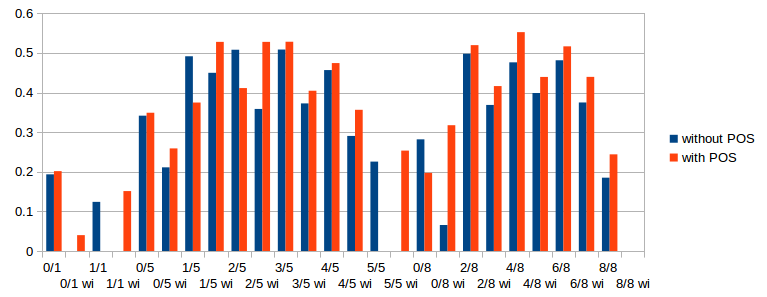
\includegraphics[width=\textwidth]{img/parameter_eval.png}
    \caption{Harmonic mean between all f1 scores for all classes. \emph{2/5} means window size of five and punctuation is tested at position two. If \emph{wi} is in the label, it uses wikipedia training data.}
    \label{fig2}
\end{figure}

Comparison between experiments with and without POS tagging (other than that, they have the same configurations):
\begin{itemize}
\item With POS tagging: 0.305
\item Without POS tagging: 0.275
\end{itemize}

Comparison between experiments with and without wikipedia data (other than that, they have the same configurations):
\begin{itemize}
\item Without wikipedia: 0.385
\item With wikipedia data: 0.252
\end{itemize}


\section{Demo Tool}
\label{sec:demo}
We use a demo application, accessible with a web browser, to present the working prototype.
It can be used to find sentence boundaries in unpunctuated text.
The general web page shows two main tabs, one labeled \emph{Lexical} and one \emph{Lexical + Audio}.
A user can click these, to switch between using only the lexical model or the fusion of both the lexical and the acoustic model.

There are two ways to feed input to our model for the \emph{Lexical} SBD (see Figure~\ref{fig:demo_l}).
\begin{figure}[ht]
    \centering
    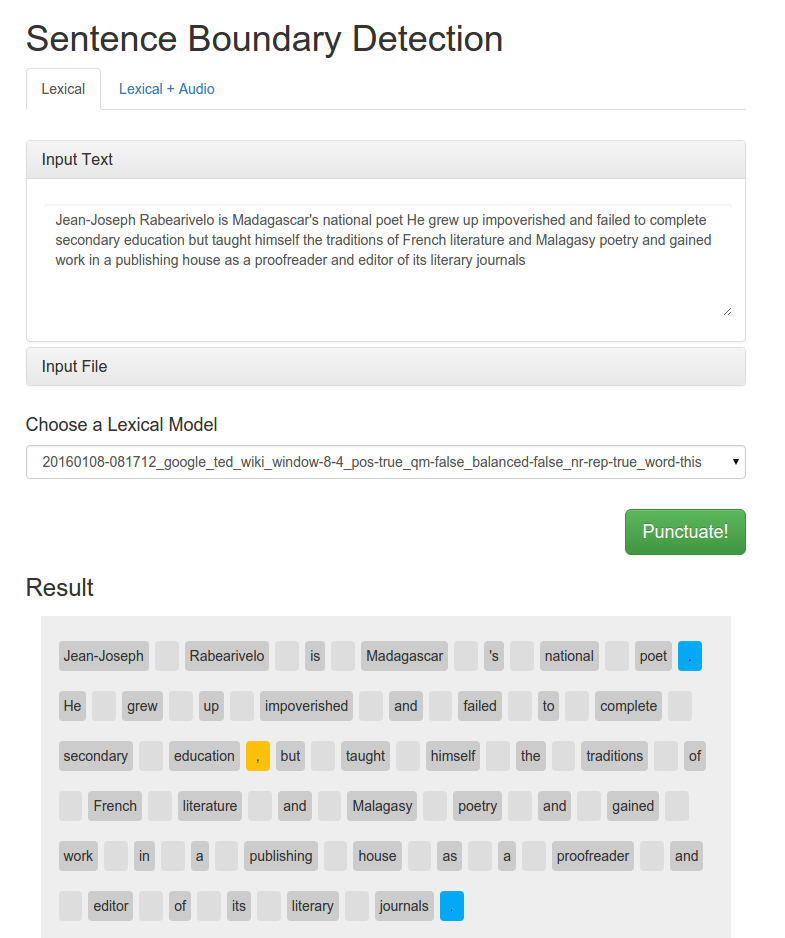
\includegraphics[width=0.5\textwidth]{img/demo_l.png}
    \caption{The demo application for lexical model. The results are presented below the options for input and model selection.}
    \label{fig:demo_l}
\end{figure}
The user can enter a text input field to manually enter or paste any text they wish.
Another possibility is to choose from a set of existing text files.
A dropdown selection allows the user to choose the pretrained models, if multiple models are available in the system.
If the model is changed, it is automatically loaded in the background.
Once the user clicks the \emph{Punctuate!} button, the text, which was entered, or selected as a file, is passed to our lexical model.
While the server processes the request, a small loading icon is shown inside the button.
After the predictions are returned from the server, the result is shown beneath.
The input text and positions where no punctuation was predicted are shown as tokens with a light grey background.
Any commas or periods inserted, are shown in distinct colors.
If a model, which uses POS tags, is selected a user can hover their mouse over a token to see its POS category.
For further use the entire result is selectable and can be copied.

For the \emph{Lexical + Audio} SBD the possibilities for entering input are more limited (see Figure~\ref{fig:demo_la}).
\begin{figure}[ht]
    \centering
    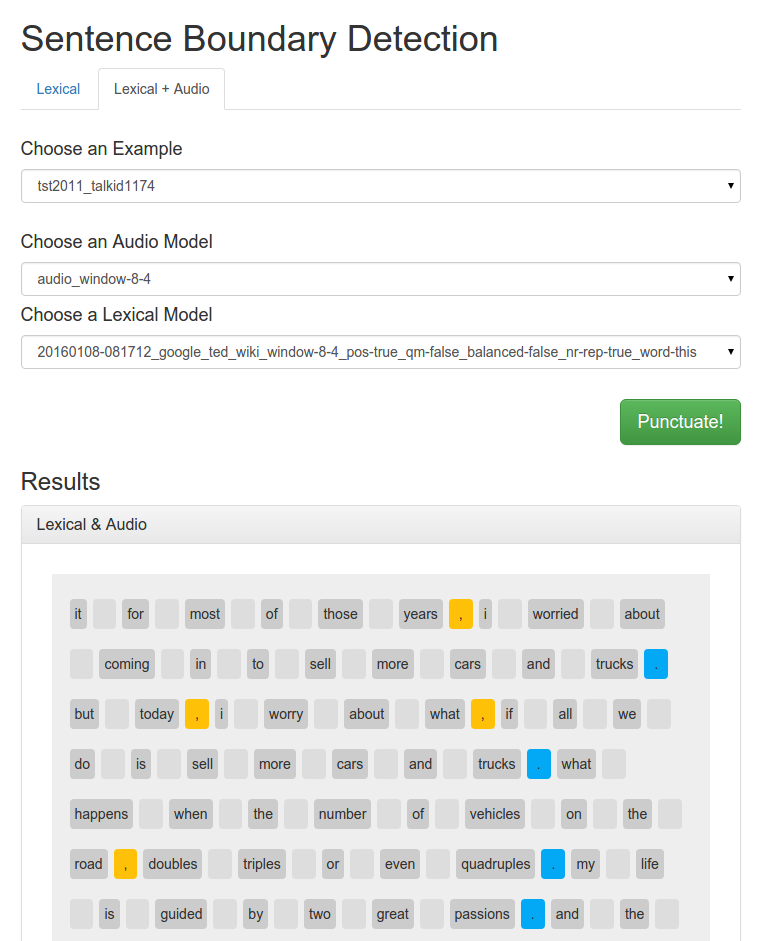
\includegraphics[width=0.5\textwidth]{img/demo_l_a.png}
    \caption{The demo application for fusion of both models. The results of the individual models and the fusion are presented below the options for input and model selection. Only one result section is in the screenshot, the other sections are out of the region of the screenshot.}
    \label{fig:demo_la}
\end{figure}
Since we need an audio recording, we only offer examples existing in the system.
At the moment the system contains samples, which were used in the testing phase, but not for training.
The selection of the user is therefore limited by a dropdown menu of all available choices.
However, the choice of both the acoustic and the lexical model is independently available to a user.
These can also be selected in a dropdown menu.
The functionality of the \emph{Punctuate!} button is unchanged.
It triggers the processing and shows a loading indicator until the result returns.
The result area however is changed, and contains three subareas, which each contain a different result.
Two of them contain the raw results of the acoustic model and the lexical model.
The third shows the result after the fusion.
Therefore, it is easy to compare the results of each individual model, and the result after the fusion.


\section{Evaluation}
\label{sec:evaluation}
% evaluation

Problem with audio data:
Not tokenized in the same way as our data
No commas
No capitalization, which is important for POS tagging


\section{Future Work}
\label{sec:future}
We presented an approach to automatically detect sentence boundaries, and predict the correct punctuation marks in unpunctuated ASR output.
Two different models were trained independently, one using lexical input and the other using acoustic input.
The results of both models were merged with a late fusion.
Evaluation has shown, that one has to be careful with the training data, which should stem only from actually spoken text.
Just adding more written text data did not improve the performance.
On the other hand, part of speech tags as additional features consistently increase the performance of the sentence boundary detection.

There are many possibilities for improvement on the presented approach.
Since we did not explore the large variety of different neural network layouts, further exploration in this area is likely to improve on the results.
Especially in the case of more training data, a deeper network architecture can provide better results.
Also, using Long Short Term Memory (LSTM) neural networks appears promising, as they can process a stream of data while keeping time information.
This maps easily to the stream of word tokens in a text.

In the fusion step we decided for a late fusion approach, which combines only the predictions.
However, another way to explore, is an earlier fusion, where both models and the fusion itself are trained together.
Instead of fusing the predictions, the actual features can be fused.
As for data preparation, a different representation of features in the lexical model can be examined, such as a second or third data channel or a combination similar to the fusion of the acoustic and lexical model.

Another improvement could be achieved with a better post processing of the results.
For example, one punctuation symbol right after another is unlikely to be correct.

\bibliographystyle{plain}
\bibliography{bibliography.bib}

\newpage
\appendix
\section{Appendix}
We appended the following files for reference:
\begin{itemize}
	\item solver.prototxt, The configuration of the solver
\end{itemize}

\subsection{solver.prototxt}
\lstinputlisting[caption={solver.prototxt}, label={lst:solver.prototxt}]{appendix/solver.txt}
%\newpage %for more appended files

\end{document}
